% fig_trajectory_placeholder.tex
% PLACEHOLDER: Relay trajectory for representative HIF case
% Rf = 72 ohm, 3PH, 0-degree inception
% Traces (normalised): M(t), gamma(t), TMS(t)/TMS_0
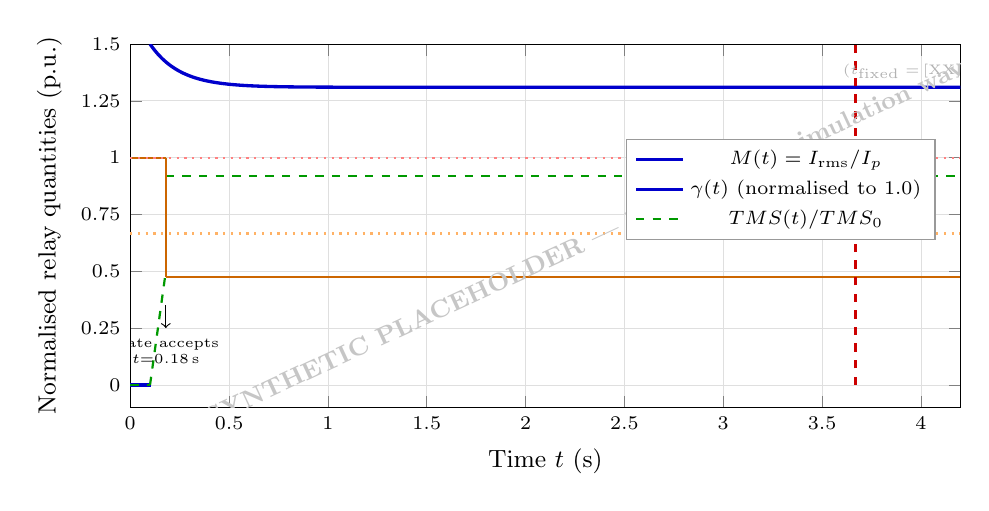
\begin{tikzpicture}
\begin{axis}[
  width=\columnwidth, height=6.2cm,
  xlabel={Time $t$ (s)},
  ylabel={Normalised relay quantities (p.u.)},
  xmin=0.0, xmax=4.2,
  ymin=-0.1, ymax=1.5,
  xtick={0,0.5,1.0,1.5,2.0,2.5,3.0,3.5,4.0},
  ytick={0,0.25,0.5,0.75,1.0,1.25,1.5},
  grid=both,
  grid style={gray!25,line width=0.3pt},
  tick label style={font=\scriptsize},
  label style={font=\small},
  legend style={at={(0.97,0.60)},anchor=east,
                font=\scriptsize,fill=white,draw=black!40},
  clip=true]

  % ---- M(t) — normalised current multiple ----
  % Pre-fault: 0; fault at t=0.1: step up to 1.31, then decay via tau_ac
  \addplot[blue!80!black,very thick,samples=200,domain=0.0:0.10]
    { 0.0 };
  \addplot[blue!80!black,very thick,samples=200,domain=0.10:4.2]
    { 1.31 + 0.19*exp(-(x-0.10)/0.15) };
  \addlegendentry{$M(t)=I_{\mathrm{rms}}/I_p$}

  % ---- gamma(t) — confidence score ----
  \addplot[green!60!black,thick,dashed,domain=0.0:0.10]
    coordinates {(0,0)(0.10,0)};
  \addplot[green!60!black,thick,dashed,samples=60,domain=0.10:0.18]
    { 0.5*(x-0.10)/0.08 };
  \addplot[green!60!black,thick,dashed,domain=0.18:4.2]
    coordinates {(0.18,0.92)(4.2,0.92)};
  \addlegendentry{$\gamma(t)$ (normalised to 1.0)}

  % ---- TMS(t)/TMS_0 ----
  \addplot[orange!80!black,thick,domain=0.0:0.18]
    coordinates {(0,1.0)(0.18,1.0)};
  % Step down at gate acceptance
  \addplot[orange!80!black,thick]
    coordinates {(0.18,1.0)(0.18,0.475)};
  \addplot[orange!80!black,thick,domain=0.18:4.2]
    coordinates {(0.18,0.475)(4.2,0.475)};
  \addlegendentry{$TMS(t)/TMS_0$}

  % gamma_min threshold
  \draw[orange!60,dotted,thick]
    (axis cs:0,0.667) -- (axis cs:4.2,0.667)
    node[right,font=\tiny,orange!60]{$\gamma_{\min}/\gamma_{\max}=0.80$};

  % M=1 pickup line
  \draw[red!50,dotted,thick]
    (axis cs:0,1.0) -- (axis cs:4.2,1.0)
    node[right,font=\tiny,red!50]{$M=1$ (pickup)};

  % Gate acceptance annotation
  \draw[->]
    (axis cs:0.18,0.35) -- ++(0,-0.20)
    node[below,font=\tiny,align=center]{Gate accepts\\$t{=}0.18$\,s};

  % Adaptive trip marker
  \draw[red!80!black,very thick,dashed]
    (axis cs:3.67,0) -- (axis cs:3.67,1.5)
    node[above,font=\tiny,red!80!black]{$t_{\mathrm{adapt}}=$\,{[XX]}\,s};

  % Fixed-TMS trip reference
  \node[font=\tiny,gray!60,align=center]
    at (axis cs:3.95,1.38)
    {($t_{\mathrm{fixed}}=$\,{[XX]}\,s)};

  % PLACEHOLDER
  \node[font=\small\bfseries,gray!45,rotate=25,align=center]
    at (axis cs:2.5,0.7)
    {SYNTHETIC PLACEHOLDER --- Replace with simulation waveforms};

\end{axis}
\end{tikzpicture}
